\part{Using HPC}
\begin{frame}
\partpage
\end{frame}
%%%%%%
\section{Connecting}
\begin{frame}{Basics: Connecting}
\begin{itemize}
\item When connecting to the cluster will we use the SSH secure protocol only.\hfill\\
\item{We will use the Linux workstations during this course}
\item{Please check your workstation is booted into Ubuntu Linux, ask if you need help with this.}
\item{You are welcome to use your own laptop, however you may need to install some software in order to connect.}
\item{Later in this section of the slides we will cover the software you may need to install on your own computer.}
\end{itemize}
\end{frame}

\subsection{Connecting - SSH}
\begin{frame}{Basics: Connecting}
\begin{itemize}
\item SSH secure protocol only.\hfill\\
\visible<2->{\alert{Supports login, file transfer, remote desktop\ldots}}
\item<3-> HPCS allows access from registered IP addresses only.\hfill\\
\visible<4->{\alert{Almost all Cambridge University addresses already registered.}}
\visible<5->{\alert{Connection from home possible via the VPN service\hfill\\
\qquad http://www.ucs.cam.ac.uk/vpn}}\hfill\\
\visible<6->{\qquad\alert{or SSH tunnel through a departmental gateway.}}
\end{itemize}
\end{frame}

\subsection{Linux Clients}
\begin{frame}{Connecting: Linux Clients}
\begin{itemize}
\item {\color<2->{red}ssh}, scp, sftp, {\color<2->{red}rsync}\hfill\\
\alert{\small Installed (or installable), in Ubuntu we will use 'Terminal'.}
\item {X Windows, for using graphical applications remotely}
\alert{\small This is already installed on your desktop.}
\end{itemize}
\end{frame}

\subsection{Login}
\begin{frame}{Connecting: Login}
\begin{itemize}
\item From Linux/MacOSX/UNIX (or Cygwin):\hfill\\
\alert{ssh -Y \textbf{abc123}@login.hpc.cam.ac.uk}
\pause
\item From graphical clients:\hfill\\
Host: \alert{login.hpc.cam.ac.uk}\hfill\\
Username: \alert{\textbf{abc123}} (your UCAM account name)
\pause
\item login.hpc will map to a random login node\hfill\\
\alert{i.e. one of login-sand1, login-sand2,\,\ldots\,, login-sand8}\hfill\\
\uncover<4->{{\color{red}NB Not darwin.hpc (the head node).}}
\item<5->Non-registered addresses will fail with ``Connection refused''.
\item<6->Similarly for other systems (e.g.\ cardio-login.hpc, login-mrc-bsu.hpc,\ldots). 
\end{itemize}
\end{frame}

\subsection{First time login}
\begin{frame}{Connecting: First time login}
\begin{itemize}
\item{The first connection to a particular hostname produces the following:}
\begin{semiverbatim}\footnotesize
The authenticity of host 'login-sand2.hpc.cam.ac.uk (131.111.1.214)' can't be established.

RSA key fingerprint is

{\color<2->{red}0b:ef:59:90:fb:13:4a:c9:56:82:7b:cd:4b:2b:e1:3b}.

Are you sure you want to continue connecting (yes/no)? {\color<3->{red}yes}

Warning: Permanently added 'login-sand2.hpc.cam.ac.uk' (RSA) to the list of known hosts.
\end{semiverbatim}
\smallskip\item{\alert{One should always check the fingerprint before typing ``yes''.}}
\item{Graphical SSH clients \emph{should} ask a similar question.}
\item{Designed to detect fraudulent servers.}
\end{itemize}
\end{frame}

\begin{frame}[fragile]{Connecting: First time login}
\begin{itemize}
\item{You may be presented with any of the following fingerprints (depending on your client):}
\begin{semiverbatim}\footnotesize

MD5:0b:ef:59:90:fb:13:4a:c9:56:82:7b:cd:4b:2b:e1:3b
SHA256:sSkVfzpwjwiFvxLcdPoDpN8IsN3kt0ZSywhDhPKZPAg

MD5:34:9b:f2:d2:c6:b3:5c:63:99:b7:27:da:5b:c8:16:fe
SHA256:HsiY1Oe0M8tS6JwR76PeQQA/VB7r8675BzG5OYQ4h34

MD5:64:7c:7c:ff:05:9d:0e:dc:06:fe:f1:c2:10:37:7a:85
SHA256:wq9ljBfPa7lXXpQq+rk5JTBXLJO/kXjOc5A7rp4ENzA

\end{semiverbatim}
\end{itemize}
\end{frame}

\subsection{File Transfer with rsync: an example}
\begin{frame}{Connecting: File Transfer}
\begin{itemize}
\item From Linux/MacOSX/UNIX (or Cygwin):\hfill\\
\alert{\footnotesize rsync -av \textbf{old\_directory/} abc123@login.hpc.cam.ac.uk:scratch/new\_directory}\hfill\\
copies contents of old\_directory to $\tilde{}\text{/scratch/new\_directory}$.\hfill\\\smallskip
\pause
\alert{\footnotesize rsync -av \textbf{old\_directory} abc123@login.hpc.cam.ac.uk:scratch/new\_directory}\hfill\\
copies old\_directory (and contents) to $\tilde{}\text{/scratch/new\_directory/old\_directory}$.\hfill\\
\pause
\item[$\ast$]For transfers in the opposite direction, place the remote machine as the first argument.
\end{itemize}
\end{frame}
%
\section{Connecting from other clients}
\begin{frame}{Basics: Connecting from other clients}
\begin{itemize}
\item{When using your own computer you you may need to install some software in order to connect.}
\pause
\item{There are quite a few choices of software packages for this, we will just cover a few.}
\pause
\item{Our website https://www.hpc.cam.ac.uk/using-clusters/connecting covers this in more detail.}
\end{itemize}
\end{frame}

\subsection{MacOSX}
\begin{frame}{Connecting: MacOSX/UNIX Clients}
\begin{itemize}
\item {\color<2->{red}ssh}, scp, sftp, {\color<2->{red}rsync}\hfill\\
\alert{\small Installed (or installable) OS X has a native terminal package. This can be launched by clicking Apple \textgreater Go \textgreater Utilities and then clicking the Terminal icon.}
\item<3-> TurboVNC \alert{\small (for remote desktop, 3D optional)}\hfill\\
\alert{\small http://sourceforge.net/projects/turbovnc/files/}
\item<4-> On MacOSX, install \alert{XQuartz} to display remote graphical applications.\hfill\\
\alert{\small http://xquartz.macosforge.org/landing/}
\end{itemize}
\end{frame}

\subsection{Windows Users}
\begin{frame}{MobaXterm SSH (Windows)}
\begin{center}
\centerline{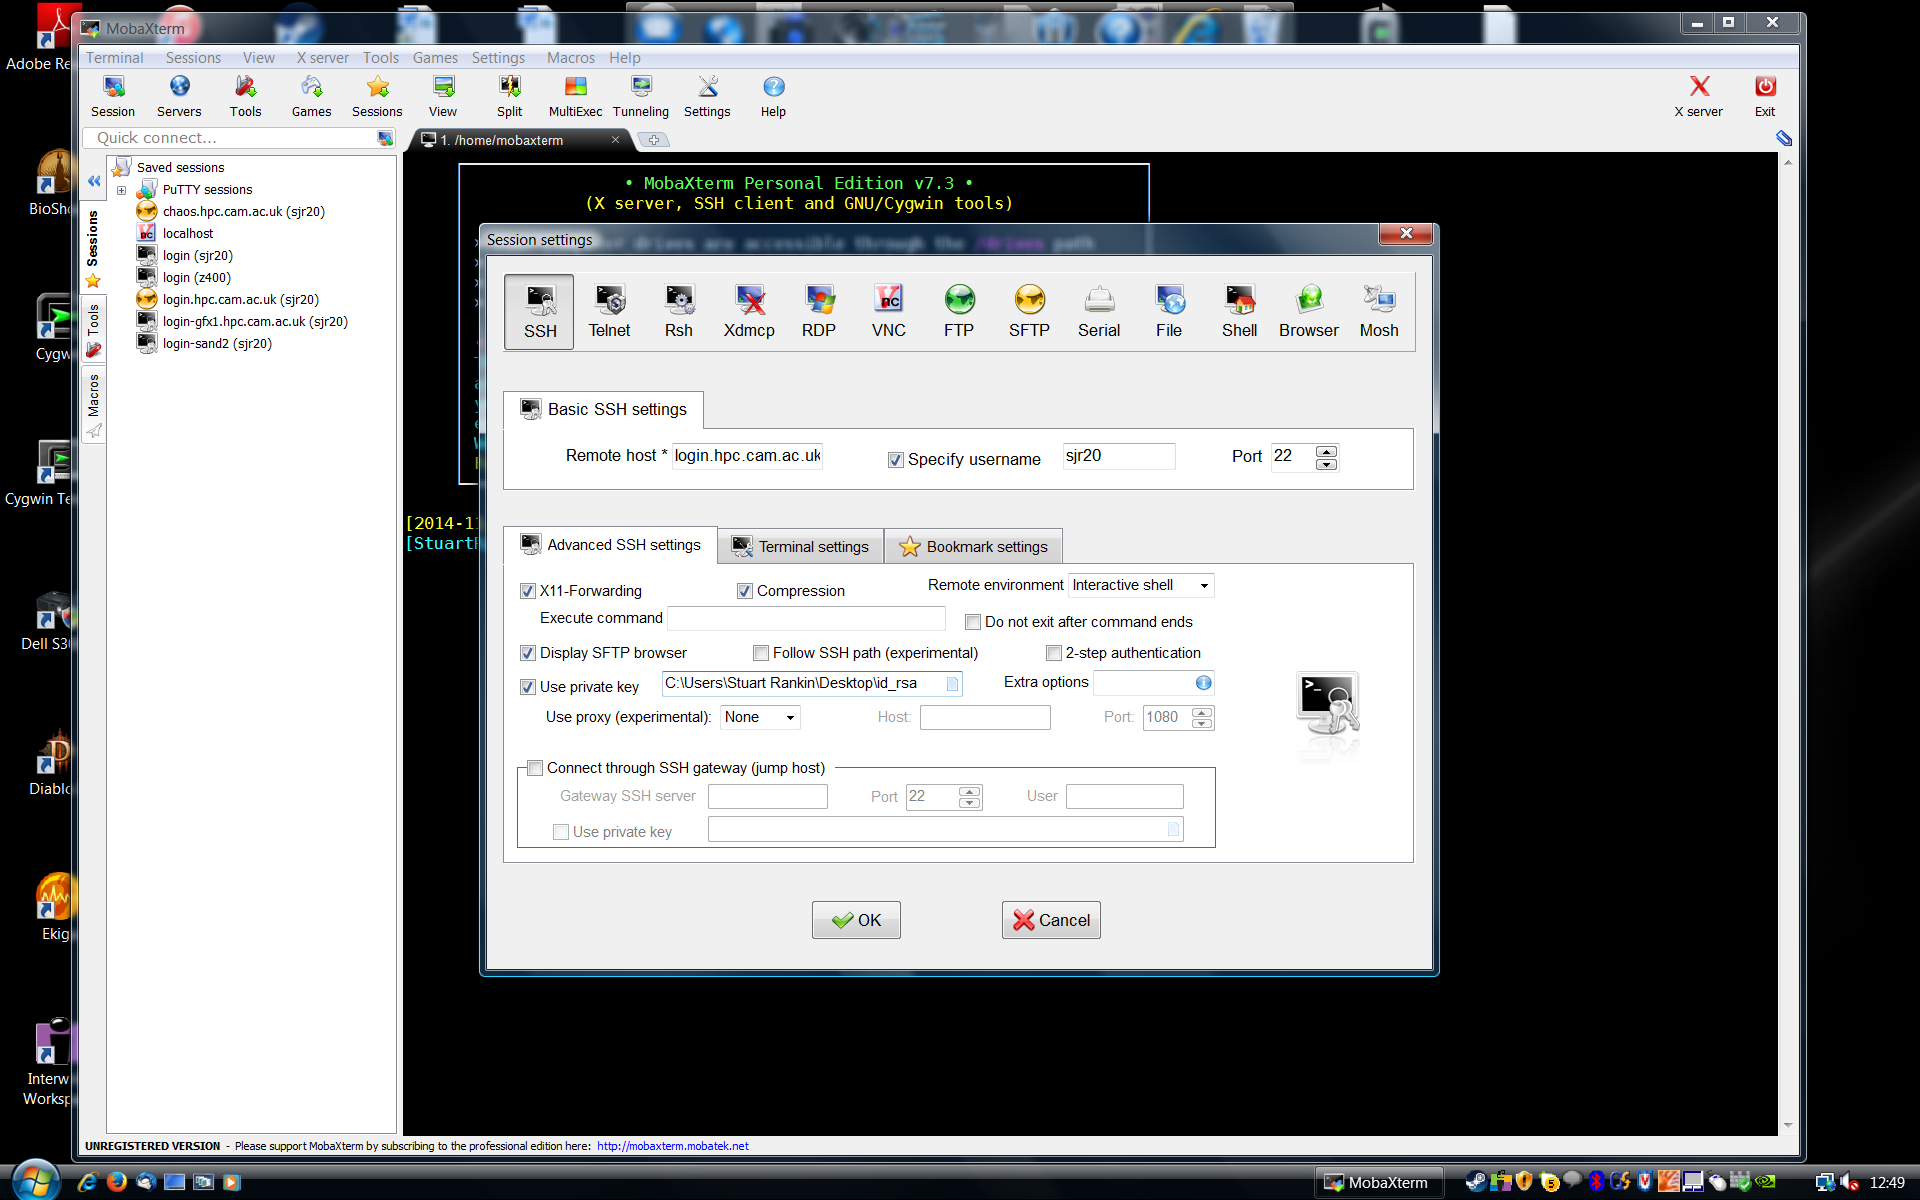
\includegraphics[height=0.8\textheight]{imgs/mobaxterm-SSH-settings2.png}}
\end{center}
\end{frame}

\begin{frame}{MobaXterm SSH (Windows)}
\begin{center}
\centerline{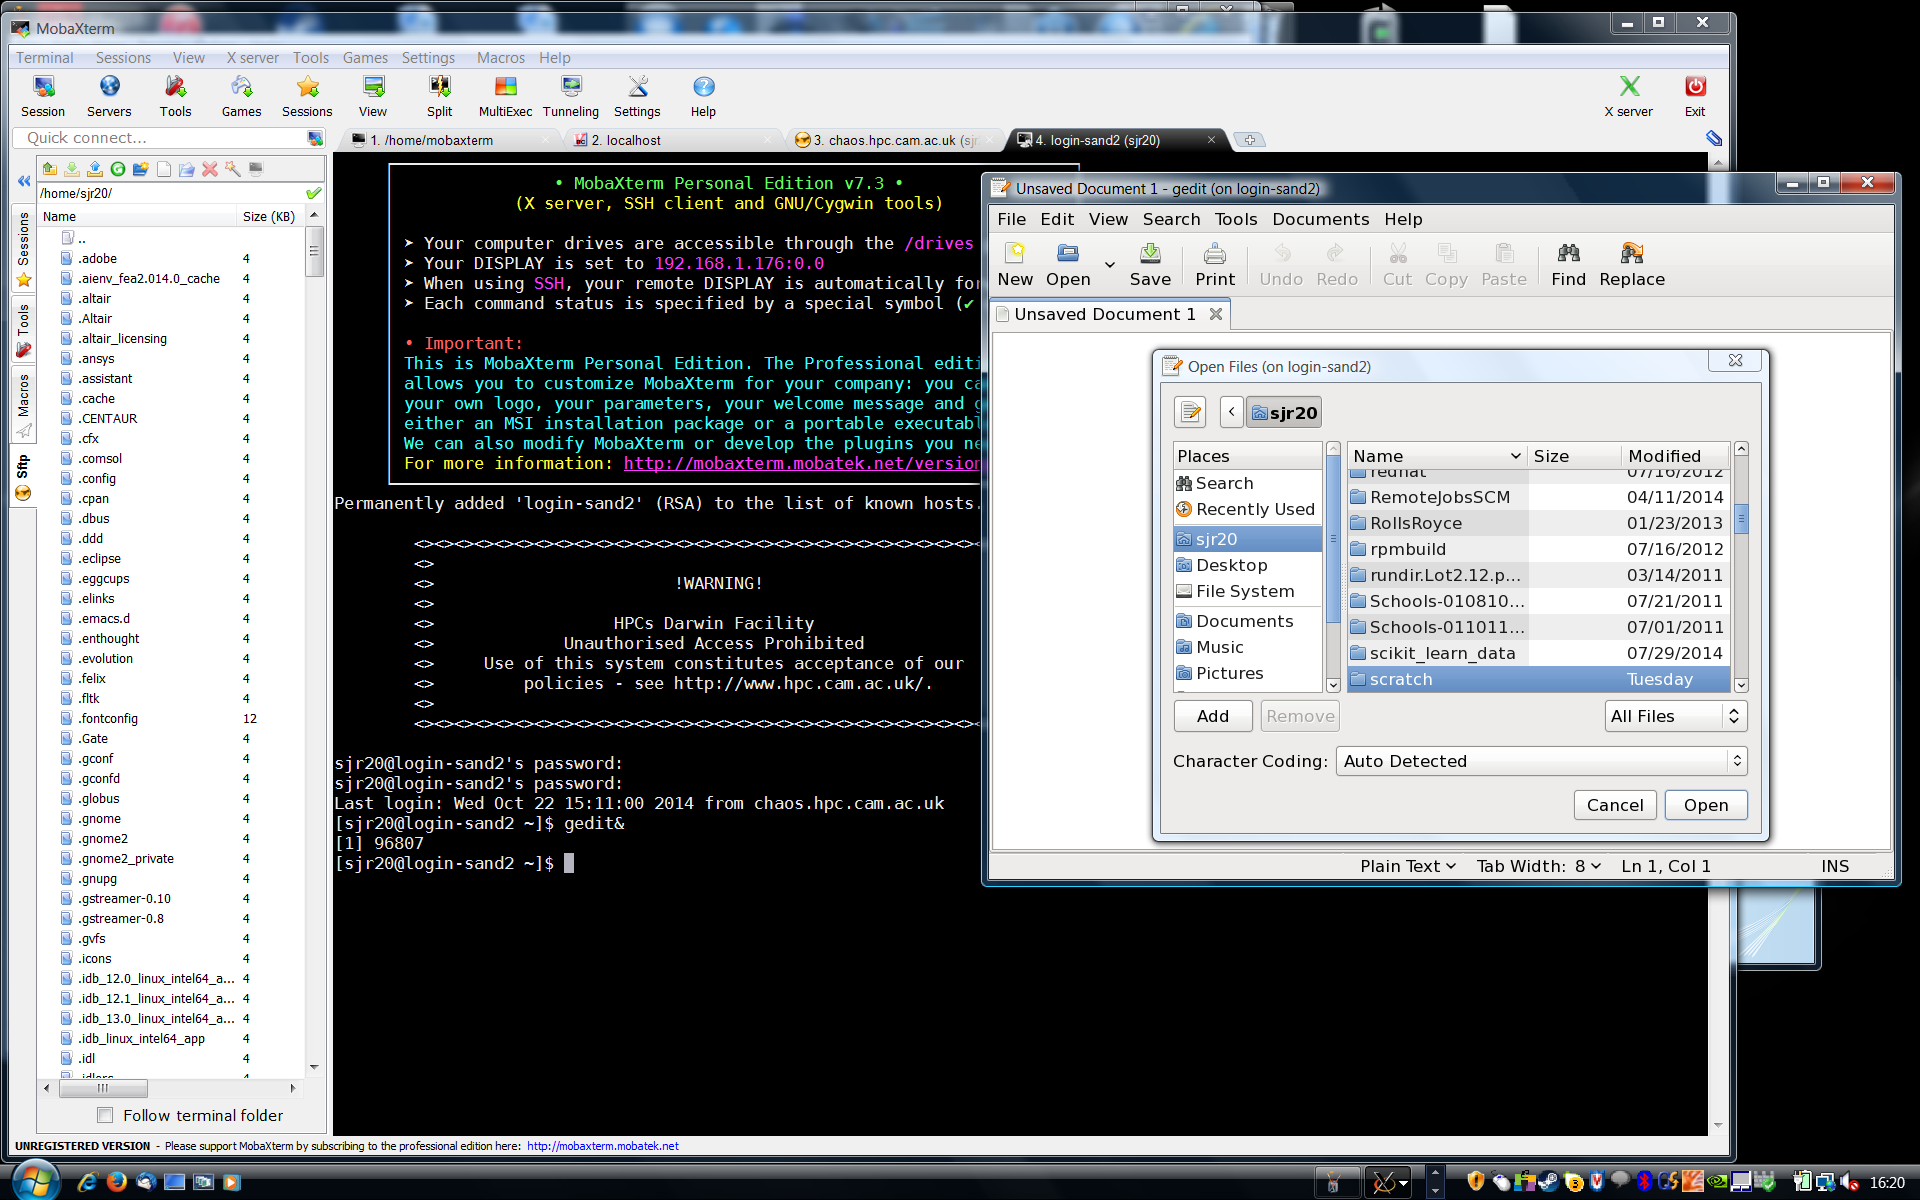
\includegraphics[height=0.8\textheight]{imgs/mobaxterm-SSH-session.png}}
\end{center}
\end{frame}

\section{Basic practicals}
\begin{frame}{Basics: A practical example before some theory}
\begin{itemize}
\item{Some simple exercises will help us gauge your experience.}
\item{Exercise 1: Login with SSH.}
\item{Exercise 2: Navigating the command line.}
\item{Exercise 3: SFTP file transfer.}
\end{itemize}
\end{frame}

\subsection{Exercise 1: Navigating the command line}
\begin{frame}{Exercise 1: Navigating your terminal}
\begin{itemize}
\item{Start a terminal by double clicking on the terminal icon}
\item{Try the \alert{\footnotesize ls } and \alert{\footnotesize cd } commands in a terminal.}
\item{Look at the man page for the ls command}
\item{Close the terminal}
\end{itemize}
\end{frame}

\subsection{Exercise 2: Login}
\begin{frame}{Exercise 2: Login}
Using a Linux terminal you will login to the cluster with your HPC training account.
\begin{itemize}
\item{Start the terminal by double clicking on the terminal icon}
\item In your terminal enter:
\item{ssh -Y \textbf{abc123}@login.hpc.cam.ac.uk}\\
Replace abc123 with your training account username 
\item {Enter your password as supplied on the sheet}
\item{Leave this terminal open, you will need it for exercise 3!}
\end{itemize}
\end{frame}

%%%%
\subsection{Exercise 3: SFTP file transfer - pt1}
\begin{frame}{Exercise 3: Transfer some files}
You will need to transfer the exercise files to the cluster.
\begin{itemize}
\item{Open a second Linux terminal on your training computer.}
\item{Enter this command: cd \alert{\footnotesize \path{~\Course_material}}}
\item{Check the file 'exercises.tar.gz is in your directory listing}
\item{Hint: ls}
\end{itemize}
\end{frame}

\subsection{Exercise 3: SFTP file transfer - pt2}
\begin{frame}{Exercise 3: Transfer some files}
Transfer the exercises.tar.gz to your HPC home folder.
\begin{itemize}
\item \alert{\footnotesize sftp abc123@login.hpc.cam.ac.uk}\\
Change abc123 to your training account username
\item{The command: \alert{\footnotesize put exercises.tar.gz} will transfer the file from your local computer to the remote one}
\item{In terminal logged into the cluster type: ls}
\item{Use: tar -xvf exercise.tar  - to unzip the file}
\end{itemize}
\end{frame}

\subsection{File Transfer with rsync}
\begin{frame}{Connecting: File Transfer}
In exercise 3 we used sftp. Another tool to be familiar with is rsync especially when you want to transfer lots of directories and files.
\begin{itemize}
\item{rsync is a powerful tool and has many features.}
\item[$\ast$]You can rerun it to update or resume after interruption.
\item[$\ast$]All transfers are checksummed.
\end{itemize}
\end{frame}
%%%%%%
\section{Connecting}
\begin{frame}{Using HPC: Connecting}
\begin{itemize}
\item SSH secure protocol only.\hfill\\
\visible<2->{\alert{Supports login, file transfer, remote desktop\ldots}}
\end{itemize}
\end{frame}

\subsection{Windows Clients}
\begin{frame}{Connecting: Windows Clients}
\begin{itemize}
\item<1-5> putty, pscp, psftp\hfill\\
\alert{\small http://www.chiark.greenend.org.uk/~sgtatham/putty/download.html}
\item<2-5> WinSCP\hfill\\
\alert{\small http://winscp.net/eng/download.php}
\item<3-5> TurboVNC \alert{\small (remote desktop, 3D optional)}\hfill\\
\alert{\small http://sourceforge.net/projects/turbovnc/files/}
\item<4-5> Cygwin \visible<5>{\alert{\small (provides an application environment similar to Linux)}}\hfill\\
\alert{\small http://cygwin.com/install.html}\hfill\\
\visible<5>{\alert{\small Includes X server for displaying graphical applications running remotely.}}
\item<6> MobaXterm\hfill\\
\alert{\small http://mobaxterm.mobatek.net/}
\end{itemize}
\end{frame}

\subsection{Linux/MacOSX/UNIX Clients}
\begin{frame}{Connecting: Linux/MacOSX/UNIX Clients}
\begin{itemize}
\item {\color<2->{red}ssh}, scp, sftp, {\color<2->{red}rsync}\hfill\\
\alert{\small Installed (or installable).}
\item<3-> TurboVNC \alert{\small (remote desktop, 3D optional)}\hfill\\
\alert{\small http://sourceforge.net/projects/turbovnc/files/}
\item<4-> On MacOSX, install \alert{XQuartz} to display remote graphical applications.\hfill\\
\alert{\small http://xquartz.macosforge.org/landing/}
\end{itemize}
\end{frame}

\subsection{Login}
\begin{frame}{Connecting: Login}
\begin{itemize}
\item From graphical clients:\hfill\\
Host: \alert{login-cpu.hpc.cam.ac.uk}\hfill\\
Username: \alert{\textbf{npl$\backslash$abc123}} (your NPL AD account name)
\pause
\item From Linux/MacOSX/UNIX (or Cygwin):\hfill\\\medskip
  \alert{ssh -Y \textbf{npl$\backslash\backslash$abc12}@minerva-login1.npl.co.uk}\hfill\\\medskip
  Note the double backslash --- this is because UNIX command interpreters treat $\backslash$ as special.
\end{itemize}
\end{frame}

\begin{frame}{Connecting: First time login}
\begin{itemize}
\item{The first connection to a particular hostname produces the following:}
\begin{semiverbatim}\tiny
The authenticity of host 'minerva-login1.npl.co.uk (139.143.201.10)' can't be established.


ECDSA key fingerprint is {\color<2->{red}SHA256:k/eB+LjcAfQW56XCzK9QptT0wVWF7j3a/CPxPRd7+lE}.

ECDSA key fingerprint is {\color<2->{red}MD5:18:9a:97:e2:87:4c:07:60:cb:43:46:f2:bb:d8:3d:01}.


Are you sure you want to continue connecting (yes/no)? {\color<3->{red}yes}

Warning: Permanently added 'minerva-login1.npl.co.uk (139.143.201.10)' (ECDSA) to the list of known hosts.
\end{semiverbatim}
\smallskip\item{\alert{One should always check the fingerprint before typing ``yes''.}}
\item{Graphical SSH clients \emph{should} ask a similar question.}
\item{Designed to detect fraudulent servers.}
\end{itemize}
\end{frame}

\begin{frame}[fragile]{Connecting: First time login}
\begin{itemize}
\item{Exercise 1 - Log into your Minerva account.}
  \pause
  \item{Exercise 2 - Simple command line operations.}
\end{itemize}
\end{frame}

\subsection{File Transfer}
\begin{frame}{Connecting: File Transfer}
\begin{itemize}
\item With graphical clients, connect as before and drag and drop.
\pause
\item From Linux/MacOSX/UNIX (or Cygwin):\hfill\\
\alert{\footnotesize rsync -av \textbf{old\_directory/} npl$\backslash\backslash$abc12@minerva-login1.npl.co.uk:hpc-work/new\_directory}\hfill\\
copies contents of old\_directory to $\tilde{}\text{/hpc-work/new\_directory}$.\hfill\\\smallskip
\pause
\alert{\footnotesize rsync -av \textbf{old\_directory} npl$\backslash\backslash$abc12@minerva-login1.npl.co.uk:hpc-work/new\_directory}\hfill\\
copies old\_directory (and contents) to $\tilde{}\text{/hpc-work/new\_directory/old\_directory}$.\hfill\\
\pause
\begin{itemize}
\item[$\ast$]Rerun to update or resume after interruption.
\item[$\ast$]All transfers are checksummed.
\item[$\ast$]For transfers in the opposite direction, place the remote machine as the first argument.
\end{itemize}
\pause
\item{Exercise 3 - File transfer.}
\end{itemize}
\end{frame}

\subsection{Remote Desktop}
\begin{frame}[fragile]{Connecting: Remote Desktop}
\begin{itemize}
\item First time starting a remote desktop:
\begin{semiverbatim}
\footnotesize
[sjr20@login-a-1 ~]\$ vncserver

You will require a password to access your desktops.

Password: 
Verify:   
Would you like to enter a view-only password (y/n)? n

New 'login-a-1:99 (sjr20)' desktop is login-a-1:{\color{red}99}

Starting applications specified in /home/sjr20/.vnc/xstartup
Log file is /home/sjr20/.vnc/login-a-1:99.log
\end{semiverbatim}
\item{NB Choose a \alert{different} password for VNC.}
\item{The VNC password protects your desktop from other users.}
\item{Remember the unique display number ({\color{red}99} here) of your desktop.}
\end{itemize}
\end{frame}

\begin{frame}[fragile]{Connecting: Remote Desktop}
\begin{itemize}
\item Remote desktop already running:
\begin{semiverbatim}
\footnotesize
[sjr20@login-a-1 ~]\$ vncserver -list

TigerVNC server sessions:

X DISPLAY #     PROCESS ID
:99             130655
\end{semiverbatim}
\smallskip\item Kill it:
\begin{semiverbatim}
\footnotesize
[sjr20@login-a-1 ~]\$ vncserver -kill :99
Killing Xvnc process ID 130655
\end{semiverbatim}
\smallskip\item\alert{Typically you only need {\color{red}one} remote desktop.}
\item\alert{Keeps running until killed, or the node reboots.}
\end{itemize}
\end{frame}

\begin{frame}[fragile]{Connecting: Remote Desktop}
\begin{itemize}
\item To connect to the desktop from Linux:\\\hfill\break
{\scriptsize
\alert{vncviewer -via npl$\backslash\backslash$abc12@minerva-login1.npl.ad.local localhost:99}}
\smallskip
\item{The display number \alert{99} will be different in general and unique to each desktop.}
\item{You will be asked firstly for your AD login password, and secondly for your VNC password.}
\item{\alert{Press F8 to bring up the control panel.}}
\pause
\item{Exercise 4 - Remote desktop (from Windows)}
\end{itemize}
\end{frame}


%\begin{frame}{TurboVNC Session}
%\begin{center}
%\centerline{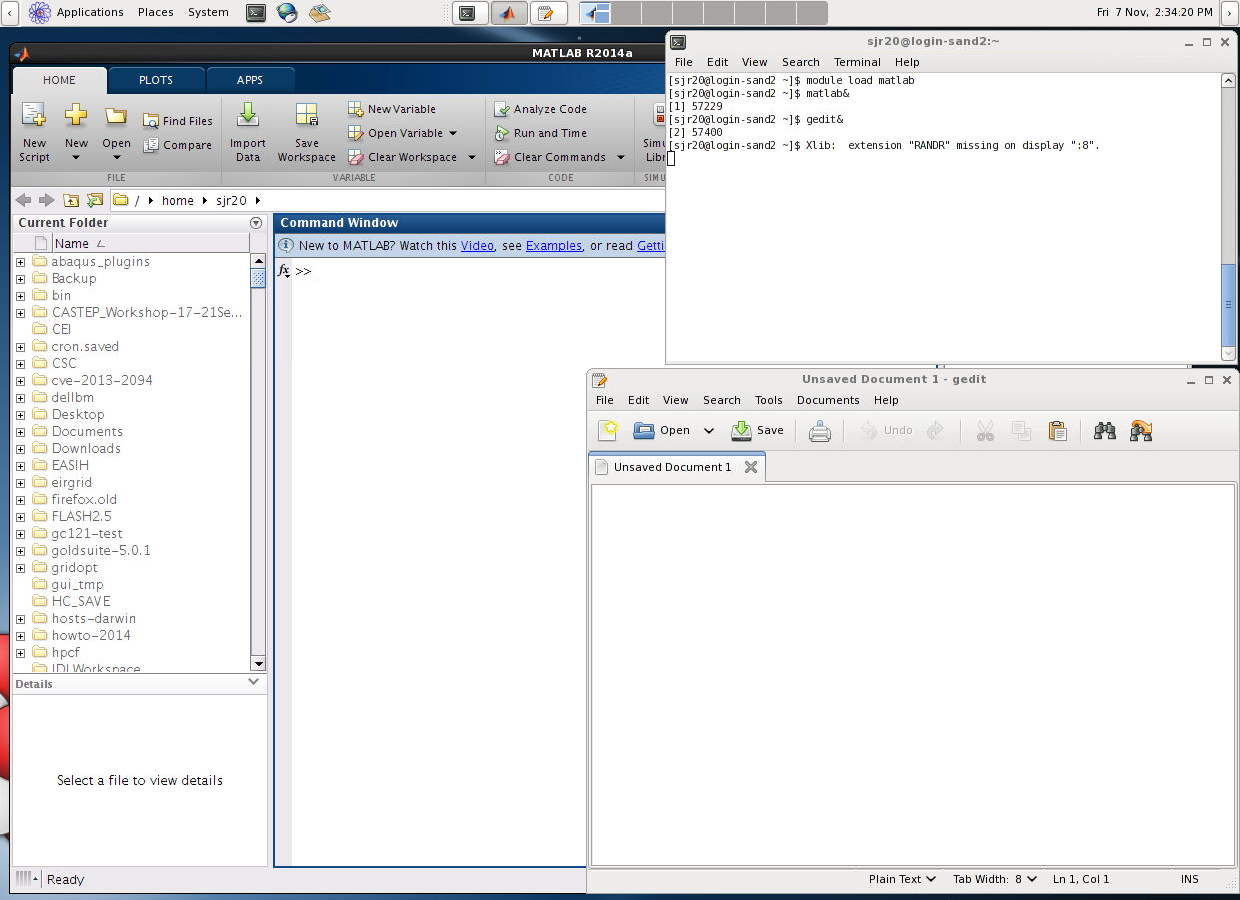
\includegraphics[width=0.85\textwidth]{imgs/linux-turbovnc.png}}
%\end{center}
%\end{frame}

%\begin{frame}{Linux TurboVNC Control Panel}
%\begin{center}
%\centerline{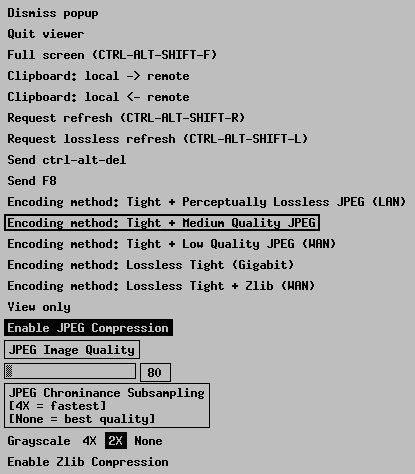
\includegraphics[height=0.8\textheight]{imgs/linux-turbovnc-F8.png}}
%\end{center}
%\end{frame}

\begin{frame}{Connecting: Remote Desktop (MobaXterm)}
\begin{center}
\centerline{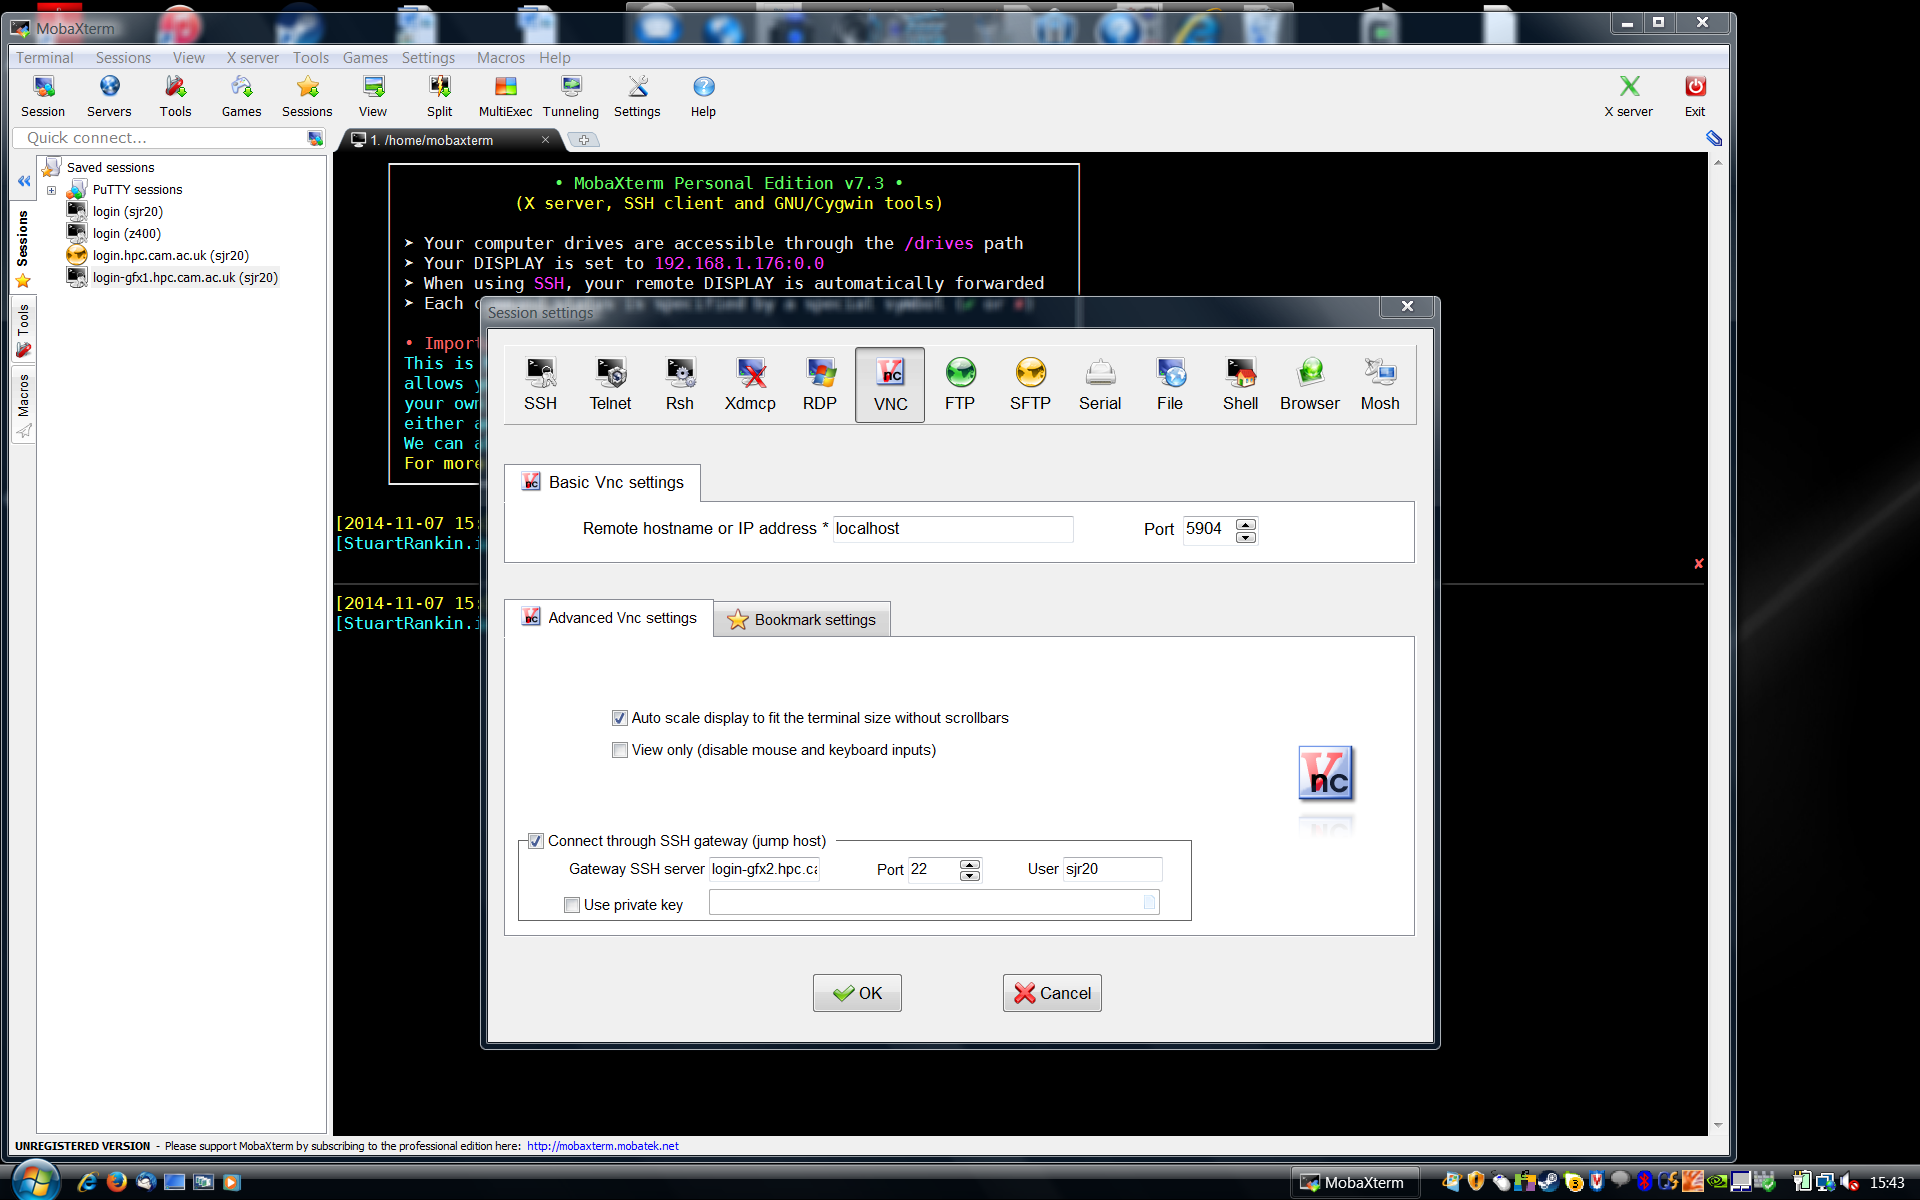
\includegraphics[height=0.8\textheight]{imgs/mobaxterm-turbovnc.png}}
\end{center}
\end{frame}

%\begin{frame}{Connecting: Remote Desktop (MobaXterm)}
%\begin{center}
%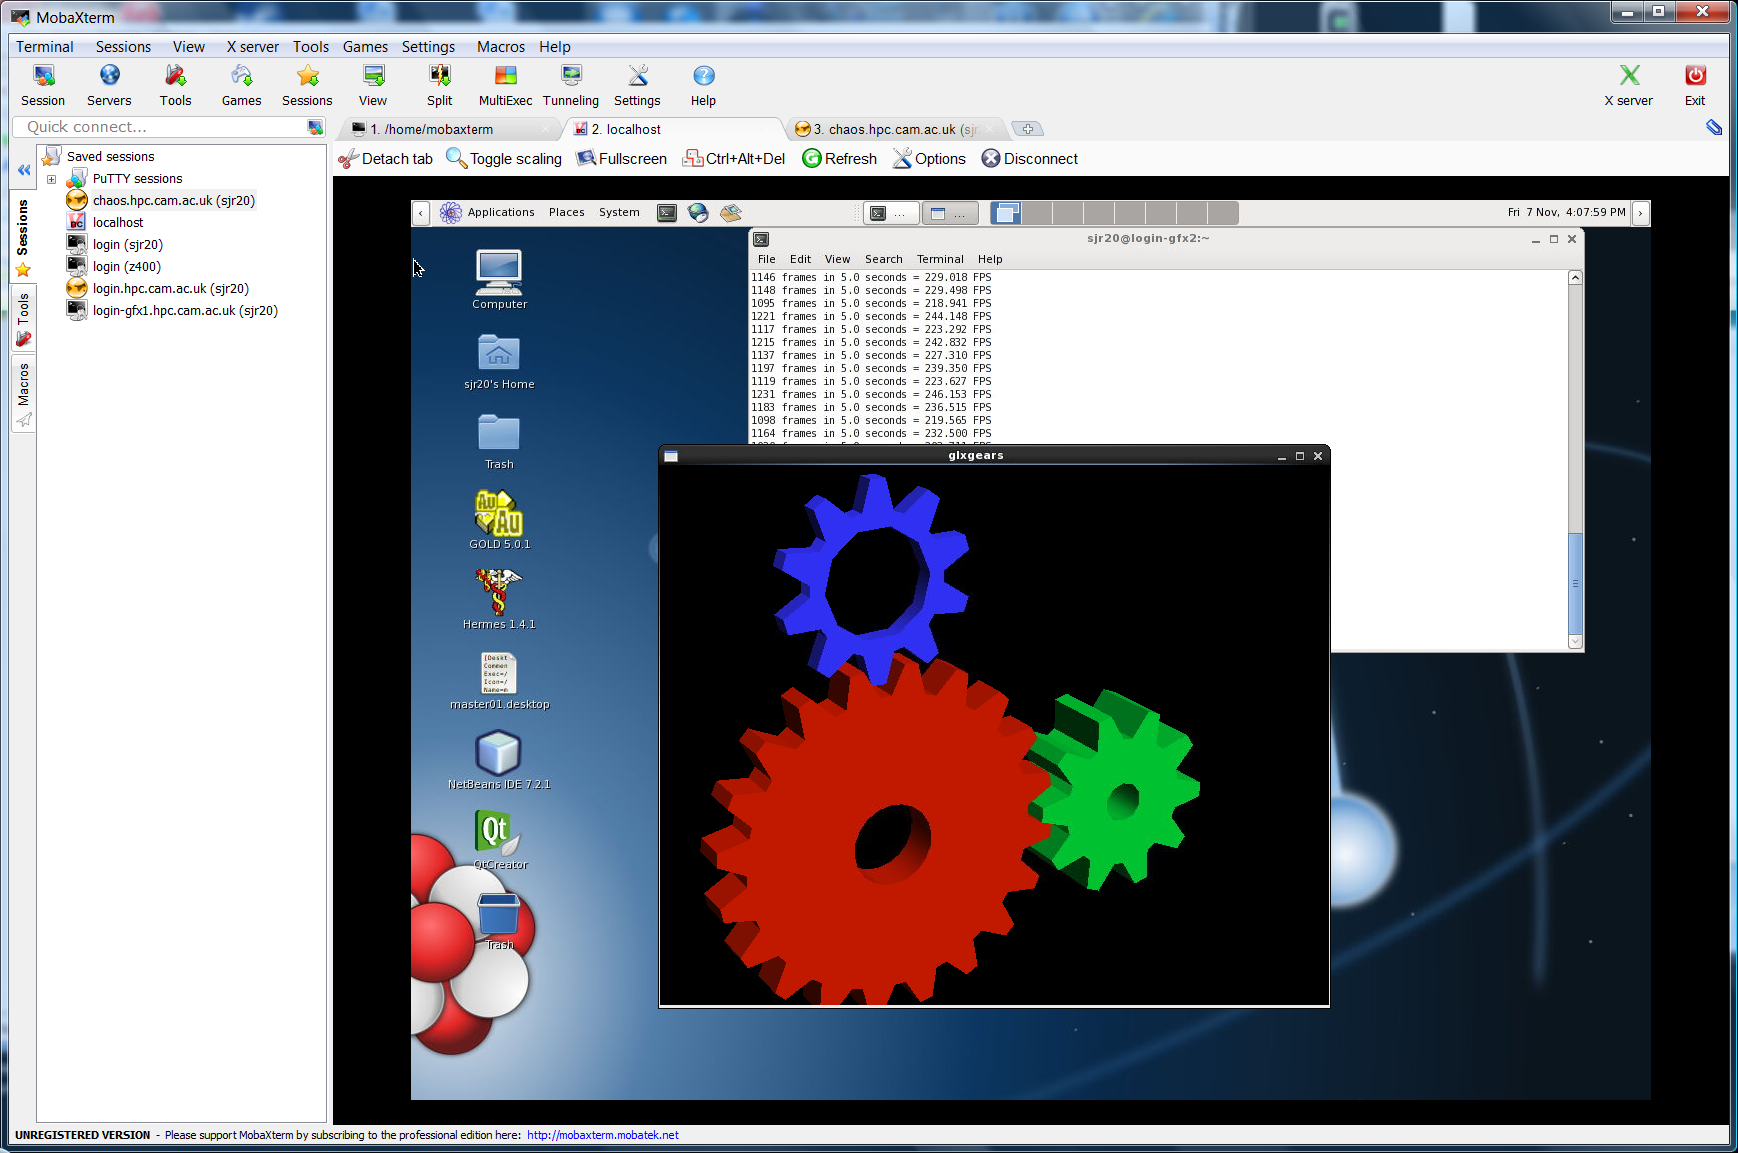
\includegraphics[height=0.8\textheight]{imgs/mobaxterm-vgl-turbovnc.png}
%\end{center}
%\end{frame}

%\begin{frame}{3D Remote Visualization}
%\begin{center}
%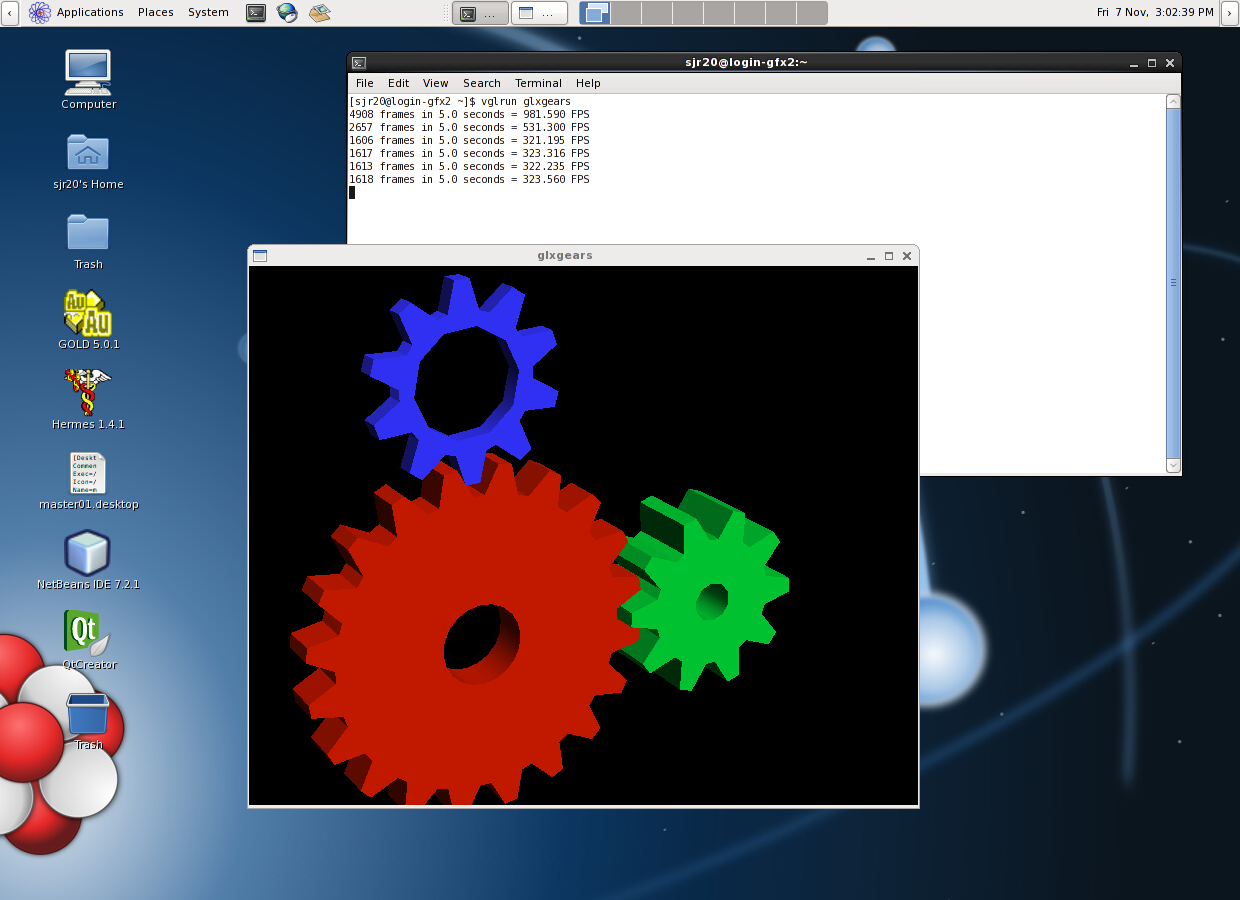
\includegraphics[height=0.8\textheight]{imgs/vgl-turbovnc.png}
%\end{center}
%\end{frame}


%12:00
%Lunch
%14:00

\section{User Environment}
\begin{frame}{Using HPC: User Environment}
\begin{itemize}
\item<1,3->{\visible<1>{CentOS Linux 7.4 (}\alert<1>{{\color<3->{red}Red Hat Enterprise Linux 7}\visible<1>{.4 rebuild)}}}
\begin{itemize}
\item{\visible<1>{bash shell}}
\item{\visible<1>{Gnome or XFCE4 desktop \alert{(if you want)}}}
\item{\visible<1>{GCC compilers and other development software.}}
\end{itemize}
\item<2->{But you don't need to know that.}
\end{itemize}
\end{frame}

\subsection{Filesystems}
\begin{frame}{User Environment: Filesystems}
\begin{itemize}
\item{\alert{/home/abc12@npl.ad.local}}
\begin{itemize}
\item{50GB quota.}
\item{Visible equally from all nodes.}
\item{Single storage server.}
\item{Regular backups.}
\item{Not intended for job outputs or large/many input files.}
\end{itemize}
\item{\alert{\~{}/hpc-work}}
\begin{itemize}
\item{Visible equally from all nodes.}
\item{Larger (1TB initial quota).}
\item{Intended for job inputs and outputs.}
\item{{\color{red}Not backed up by default.}}
\end{itemize}
\end{itemize}
\end{frame}

\begin{frame}[fragile]{Filesystems: Quotas}
\begin{itemize}
\item{quota}
\begin{semiverbatim}
\tiny
[sjr20@login-a-1 ~]$ quota -s
Disk quotas for user sjr20 (uid 1004): 
     Filesystem   space   quota   limit   grace   files   quota   limit   grace
10.44.82.252:/hpc-work
                     0K   1024G   1126G               1       0       0        
10.44.82.252:/home
                 13272K  51200M  56320M             345       0       0        
\end{semiverbatim}
\item<1-|handout:1->{\alert{Aim to stay below the soft limit (\emph{quota}).}}
\item<2-|handout:1->{\alert{Once over the soft limit, you have 7 days grace to return below.}}
\item<3-|handout:2>{\alert{When the grace period expires, or you reach the hard limit (\emph{limit}), no more data can be written.}}
\item<4-|handout:2>{\alert{It is important to rectify an out of quota condition ASAP.}}
\end{itemize}
\end{frame}

%\begin{frame}{Filesystems: Backups???}
%\begin{itemize}
%\item<1->{Disk snapshots and tape (as of May 2017).}
%\item<2->{{\color{red}They are not an undelete - take care when deleting.}}
%\item<3->{Successful restoration depends on:}
%\begin{itemize}
%\item{The file having existed long enough to have been backed up at all.}
%\item{The last good version existing in a current backup.}
%\item<4->{\color{red}Request restoration as soon as possible with \emph{location} and \emph{exact time of loss}.}
%\medskip
%\visible<5->{\item{\color{purple}\huge Scratch files are not backed up.}}
%\end{itemize}
%\end{itemize}
%\end{frame}

\begin{frame}{Filesystems: Permissions}
\begin{itemize}
\item{\color{red}Be careful and if unsure, please ask support.}
\begin{itemize}
\item{Can lead to \alert{accidental destruction} of your data or \alert{account compromise}.}
\end{itemize}
\item{Avoid changing the permissions on your home directory.}
\begin{itemize}
\item{Files under /home are particularly security sensitive.}
\item{Easy to break passwordless communication between nodes.}
\end{itemize}
\end{itemize}
\end{frame}

\subsection{Software}
\begin{frame}{User Environment: Software}
\begin{itemize}
\item{Free software accompanying \alert{Red Hat Enterprise Linux} is (or can be) provided.}
\item{Other software (free and non-free) is available via \alert{modules}.}
\item{Proprietary software currently available includes Matlab and COMSOL.}
\item{New software may be possible to provide on request.}
\item{\alert{Self-installed software should be properly licensed.}}
  \pause
\item{\color{red}\emph{sudo will not work.}\/ (You should be worried if it did.)}
\end{itemize}
\end{frame}

\subsection{Environment Modules}
\begin{frame}[fragile]{User Environment: Environment Modules}
\begin{itemize}
\item{Modules load or unload additional software packages.}
\item{Some are \alert{required} and automatically loaded on login.}
\item{Others are optional extras, or possible replacements for other modules.}
\item{\alert{Beware} unloading default modules in $\tilde{}\text{/.bashrc}$.}
\item{\alert{Beware} overwriting environment variables such as PATH and LD\_LIBRARY\_PATH in $\tilde{}\text{/.bashrc}$. If necessary append or prepend.}
\end{itemize}
\end{frame}

\subsection{Environment Modules}
\begin{frame}[fragile]{User Environment: Environment Modules}
\begin{itemize}
\item{Currently loaded:}
\begin{semiverbatim}
\scriptsize
module list
Currently Loaded Modulefiles:
  1) dot                     3) centos7/global
  2) slurm                   4) centos7/default-basic
\end{semiverbatim}
\medskip
\item{Available:}
\begin{semiverbatim}
\scriptsize
module av
\end{semiverbatim}
\end{itemize}
\end{frame}

\begin{frame}[fragile]{User Environment: Environment Modules}
\begin{itemize}
\item{Whatis:}
\begin{semiverbatim}
\tiny
module whatis openmpi-3.0.0-gcc-4.8.5-n2hvjgm
openmpi-3.0.0-gcc-4.8.5-n2hvjgm: The Open MPI Project is an open source...
\end{semiverbatim}
\medskip
\item{Load:}
\begin{semiverbatim}
\scriptsize
module load openmpi-3.0.0-gcc-4.8.5-n2hvjgm
\end{semiverbatim}
\medskip
\item{Unload:}
\begin{semiverbatim}
\scriptsize
module unload openmpi-3.0.0-gcc-4.8.5-n2hvjgm
\end{semiverbatim}
\end{itemize}
\end{frame}

\begin{frame}[fragile]{User Environment: Environment Modules}
\begin{itemize}
\item{Matlab}
\begin{semiverbatim}
\scriptsize
module load matlab/r2018a
\end{semiverbatim}
\medskip\pause
\item{Invoking matlab in batch mode:\hfill\\
  \qquad \alert{matlab -nodisplay -nojvm -nosplash command}\hfill\\
  where the file \alert{command.m} contains your matlab code.}
  \pause
  \item{The current site license contains the Parallel Computing Toolbox.}
\end{itemize}
\end{frame}

\begin{frame}[fragile]{User Environment: Environment Modules}
\begin{itemize}
\item{Purge:}
\begin{semiverbatim}
\scriptsize
module purge
\end{semiverbatim}
\smallskip
\item{Defaults:}
\begin{semiverbatim}
\scriptsize
module show centos7/default-basic
module load centos7/default-basic
\end{semiverbatim}
\medskip
\item{Run time environment must match compile time environment.}
\end{itemize}
\end{frame}

\subsection{Compilers}
\begin{frame}[fragile]{User Environment: Compilers}
  \begin{itemize}
    \item{GCC}
\begin{semiverbatim}
\scriptsize
gcc -O3 -mtune=native code.c -o prog
gfortran -O3 -mtune=native code.f90 -o prog
\medskip
module load openmpi-3.0.0-gcc-4.8.5-n2hvjgm
mpicc -O3 -mtune=native mpi_code.c -o mpi_prog
mpif90 -O3 -mtune=native mpi_code.f90 -o mpi_prog
\end{semiverbatim}
\pause
\item{Exercise 5: Modules and Compilers}
\end{itemize}
\end{frame}


%15:00
%Break
%15:15

\section{Job Submission}
\begin{frame}{Using HPC: Job Submission}
\centerline{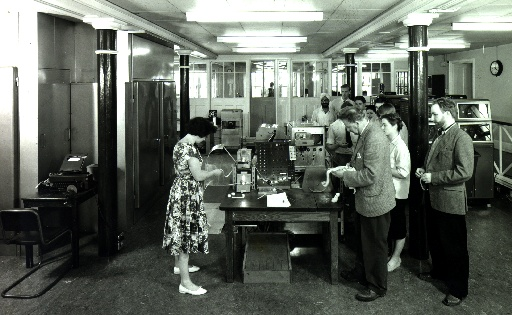
\includegraphics[width=1\textwidth]{imgs/EDSAC_2_1960.jpg}}
\end{frame}
\begin{frame}{Using HPC: Job Submission}
\begin{itemize}
\item{Compute resources are managed by a scheduler:\hfill\\\qquad\alert{SLURM}/PBS/SGE/LSF/\ldots}
\item{Jobs are submitted to the scheduler\hfill\\\qquad --- analogous to submitting jobs to a print queue\hfill\\\qquad --- a file (\emph{submission script}) is copied and queued\hfill\\\qquad \hphantom{---} for processing.}
\end{itemize}
\end{frame}

\begin{frame}{Using HPC: Job Submission}
\begin{itemize}
\item{Jobs are submitted from the \alert{login node}\hfill\\\qquad  --- not itself managed by the scheduler.}
\item{Jobs may be either non-interactive (\alert{batch}) or \alert{interactive}.}
\pause
\item{\alert{Batch} jobs run a shell script on the first of a list of allocated nodes.}
\item{\alert{Interactive} jobs provide a command line on the first of a list of allocated nodes.}
\end{itemize}
\end{frame}

\begin{frame}{Using HPC: Job Submission}
\begin{itemize}
\item{Jobs may use \alert{part} or \alert{all} of one or more nodes\hfill\\
\qquad --- the owner can specify \mbox{\tt --exclusive} to force exclusive\hfill\\\qquad\hphantom{---} node access.}
\item{Template submission scripts are available under\hfill\\
\qquad \alert{$\tilde{}$/job\_templates}.}
\end{itemize}
\end{frame}

\begin{frame}[fragile]{Job Submission: Using SLURM}
\begin{itemize}
\item{Prepare a shell script and submit it to SLURM:}
\begin{semiverbatim}
\scriptsize
[abc123@login-a-1]$ sbatch slurm_submission_script
Submitted batch job {\color{red}790299}
\end{semiverbatim}
\end{itemize}
\end{frame}

\begin{frame}[fragile]{Job Submission: Show Queue}
\begin{itemize}
\item{Submitted job scripts are copied and stored in a queue:}
\begin{semiverbatim}
\tiny
[abc123@login-a-1]$ squeue -u abc123
             JOBID PARTITION     NAME     USER ST       TIME  NODES NODELIST(REASON)
            {\color{red}790299}   skylake     Test3  abc123 PD       0:00      2 (\only<1>{{\color{blue}Priority}}\only<2>{{\color{green}Resources}}\only<3>{{\color{red}AssocGrpCPUMinsLimit}})
            790290   skylake     Test2  abc123  R   27:56:10      2 cpu-a-[1,10]
\end{semiverbatim}
\end{itemize}
\end{frame}

\begin{frame}[fragile]{Job Submission: Monitor Job}
\begin{itemize}
\item{Examine a particular job:}
\begin{semiverbatim}
\scriptsize
[abc123@login-a-1]$ scontrol show job={\color{red}790290}
\end{semiverbatim}
\end{itemize}
\end{frame}

\begin{frame}[fragile]{Job Submission: Cancel Job}
\begin{itemize}
\item{Cancel a particular job:}
\begin{semiverbatim}
\scriptsize
[abc123@login-a-1]$ scancel {\color{red}790290}
\end{semiverbatim}
\end{itemize}
\end{frame}

\begin{frame}[fragile]{Job Submission: Scripts}
\begin{itemize}
\item{SLURM\hfill\\
In \alert{$\tilde{}$/job\_templates}, see examples: \alert{slurm\_submit.skylake.generic}, \alert{slurm\_submit.skylake.matlab}.}
  
\begin{semiverbatim}
\tiny
#!/bin/bash
#! Name of the job:
{\color<2->{red}#SBATCH} -J myjob
#! Which project should be charged:
{\color<2->{red}#SBATCH} -A NPL-GENERAL-CPU
#! How many whole nodes should be allocated?
{\color<2->{red}#SBATCH} --nodes=1
#! How many tasks will there be in total? (<= nodes*32)
{\color<2->{red}#SBATCH} --ntasks={\color<3->[rgb]{1,0,0}\only<1-3>{1}\only<4->{16}}
#! How much wallclock time will be required?
{\color<2->{red}#SBATCH} --time=02:00:00
#! Select partition:
{\color<2->{red}#SBATCH} -p skylake
...
\end{semiverbatim}
\item<2->{{\color{red}\#SBATCH} lines are \emph{structured comments}\hfill\\
\qquad --- correspond to sbatch command line options.}
\item<3->{\alert{The above job will be given {\color<3->[rgb]{1,0,0}\only<1-3>{1 cpu}\only<4->{16 cpus}} on 1 node for 2 hours (by default there is 1 task per node, and 1 cpu per task).}}
\end{itemize}
\end{frame}

\begin{frame}[fragile]{Job Submission: Accounting Commands}
\begin{itemize}
\item{How many core hours available do I have?}
\begin{semiverbatim}
\tiny
mybalance

User           Usage |        Account     Usage | Account Limit Available (hours)
---------- --------- + -------------- --------- + ------------- ---------
sjr20              3 |    SUPPORT-CPU     2,929 |    22,425,600 {\color{red}22,422,671}
sjr20              0 |    SUPPORT-GPU         0 |        87,600    {\color{red}87,600}
\end{semiverbatim}
\smallskip
\item{How many core hours does some other project or user have?}
\begin{semiverbatim}
\tiny
gbalance -p SUPPORT-CPU

User           Usage |        Account     Usage | Account Limit Available (hours)
---------- --------- + -------------- --------- + ------------- ---------

pfb29          2,925 |    SUPPORT-CPU     2,929 |    22,425,600 22,422,671
sjr20 *            3 |    SUPPORT-CPU     2,929 |    22,425,600 22,422,671
...
(Use -u for user.)
\end{semiverbatim}
\smallskip
\item{List all jobs charged to a project/user between certain times:}
\begin{semiverbatim}
\Tiny
gstatement -p NPL-GENERAL-CPU  -u xyz10 -s "2018-04-01-00:00:00" -e "2018-04-30-00:00:00" 
       JobID      User    Account    JobName  Partition                 End ExitCode      State  CompHrs 
------------ --------- ---------- ---------- ---------- ------------------- -------- ---------- -------- 
263              xyz10 support-c+ _interact+    skylake 2018-04-18T19:44:40      0:0    TIMEOUT      1.0
264              xyz10 support-c+ _interact+    skylake 2018-04-18T19:48:07      0:0 CANCELLED+      0.1
275              xyz10 support-c+ _interact+    skylake             Unknown      0:0    RUNNING      0.3
...
\end{semiverbatim}
\end{itemize}
\end{frame}


\subsection{Single Node Jobs}
\begin{frame}[fragile]{Job Submission: Single Node Jobs}
\begin{itemize}
\item{Serial jobs requiring large memory, or OpenMP codes.}
\begin{semiverbatim}
\scriptsize
#!/bin/bash
\ldots
#SBATCH --nodes=1
\uncover<2-|handout:2->{{\color{red}#SBATCH --ntasks=1
# Default is 1 task per node}} 
\uncover<3-|handout:2->{{\color{red}#SBATCH --cpus-per-task=\only<3-5|handout:2>{1}\only<6,8-|handout:3,5->{32 # Whole node}\only<7|handout:4>{16  # Half node}
\only<3-5|handout:2>{# Default is 1 cpu (core) per task}}}
\uncover<4-5|handout:2>{{\color{red}#SBATCH --mem=5990
# Memory per node in MB - default is pro rata by cpu number}}
\uncover<5|handout:2>{{\color{red}# Increasing --mem or --cpus-per-task implicitly increases the other}}
\ldots
\uncover<6-|handout:3->{{\color{red}export OMP\_NUM\_THREADS=\only<6|handout:3>{32}\only<7-|handout:4->{16}  # For OpenMP across \only<6|handout:3>{32}\only<7-|handout:4->{16} cores\only<8-|handout:5->{ (using all memory)}}}
$application \$options
\ldots
\end{semiverbatim}
\end{itemize}
\end{frame}

\subsection{MPI Jobs}
\begin{frame}[fragile]{Job Submission: MPI Jobs}
\begin{itemize}
\item{Parallel job across multiple nodes.}
\begin{semiverbatim}
\scriptsize
#!/bin/bash
\ldots
#SBATCH --nodes={\color{red}4}
#SBATCH --ntasks=\alert{\only<1|handout:1>{128}\only<2-|handout:2->{64}}     # \only<1|handout:1>{i.e.\ {\color[rgb]{0,0.8,0}32}}\only<2-|handout:2->{i.e.\ {\color[rgb]{0,0.8,0} 16}}x{\color{red}4} MPI tasks in total.
\uncover<2-|handout:2->{{\color{red}#SBATCH --cpus-per-task=2}}
\ldots
mpirun\only<2-|handout:2->{ -ppn {\color[rgb]{0,0.8,0}16}} -np \alert{\only<1|handout:1>{128}\only<2-|handout:2->{64}} \$application \$options
\ldots
\end{semiverbatim}
\item<3-|handout:2->{\small SLURM-aware MPI launches remote tasks via SLURM.}
\item<3-|handout:2->{\small The template script uses \$SLURM\_TASKS\_PER\_NODE to set PPN.}
\end{itemize}
\end{frame}

\subsection{Hybrid Jobs}
\begin{frame}[fragile]{Job Submission: Hybrid Jobs}
\begin{itemize}
\item{Parallel jobs using both MPI and OpenMP.}
\begin{semiverbatim}
\scriptsize
#!/bin/bash
\ldots
#SBATCH --nodes={\color{red}4}
#SBATCH --ntasks=\alert{64}     # i.e.\ {\color[rgb]{0,0.8,0}16}x{\color{red}4} MPI tasks in total.
#SBATCH --cpus-per-task={\color{brown}2}
\ldots
{\color{brown}export OMP\_NUM\_THREADS=2   # i.e.\ 2 threads per MPI task.}
mpirun -ppn {\color[rgb]{0,0.8,0}16} -np \alert{64} \$application \$options
\ldots
\end{semiverbatim}
\item<2->{\small This job uses \alert{128 CPUs} (each MPI task splits into 2 OpenMP threads).}
\end{itemize}
\end{frame}

\subsection{High Throughput Jobs}
\begin{frame}[fragile]{Job Submission: High Throughput Jobs}
\begin{itemize}
\item{Multiple serial jobs across multiple nodes.}
\item{Use \alert{srun} to launch tasks (\alert{job steps}) within a job.}
\begin{semiverbatim}
\scriptsize
#!/bin/bash
\ldots
#SBATCH --nodes=2
\ldots
cd directory\_for\_job1
\alert{srun} {\color<3>{red}--exclusive} {\color<2>{red}-N 1 -n 1} \$application \$options\_for\_job1 > output 2> err {\color<4>{red}&}
cd directory\_for\_job2
\alert{srun} {\color<3>{red}--exclusive} {\color<2>{red}-N 1 -n 1} \$application \$options\_for\_job2 > output 2> err {\color<4>{red}&}
...
cd directory\_for\_job64
\alert{srun} {\color<3>{red}--exclusive} {\color<2>{red}-N 1 -n 1} \$application \$options\_for\_job64 > output 2> err {\color<4>{red}&}
{\color<5>{red}wait}
\end{semiverbatim}
\item<6>{Exercise 6 - Submitting Jobs.}
\end{itemize}
\end{frame}

\subsection{Interactive Jobs}
\begin{frame}[fragile]{Job Submission: Interactive}
\begin{itemize}
\item{Compute nodes are accessible via SSH \alert{while you have a job running on them}.}
\pause
\item{Alternatively, submit an interactive job:}
\begin{semiverbatim}
\alert{sintr -A NPL-GENERAL-CPU -N1 -n8 -t 2:0:0}
\end{semiverbatim}
\medskip
\pause
\item{Within the window (screen session):}
\begin{itemize}
\item[$\ast$]{Launches a shell on the first node (when the job starts).}
\item[$\ast$]{Graphical applications should display correctly.}
\item[$\ast$]{Create new shells with \alert{ctrl-a c}, navigate with \alert{ctrl-a n} and \alert{ctrl-a p}.}
\item[$\ast$]{\alert{ssh} or \alert{srun} can be used to start processes on any nodes in the job.}
\item[$\ast$]{SLURM-aware MPI will do this automatically.}
\end{itemize}
\end{itemize}
\end{frame}


\subsection{Array Jobs}
\begin{frame}[fragile]{Job Submission: Array Jobs}
\begin{itemize}
\item{\alert{$http://slurm.schedmd.com/job\_array.html$}}
\item{Used for submitting and managing large sets of similar jobs.}
\item{Each job in the array has the same \alert{initial} options.}
\item{SLURM}
\begin{semiverbatim}
\scriptsize
[abc123@login-a-1]$ sbatch --array=\only<1,2>{{\color{red}1-7}}\only<2>{{\color{red}:2}}\only<3->{{\color{red}1,3,5,7}} -A NPL-GENERAL-CPU submit\_script
Submitted batch job {\color[rgb]{0,0.6,0}791609}
\tiny
\uncover<4->{[abc123@login-a-1]$ squeue -u abc123
             JOBID PARTITION     NAME     USER ST       TIME  NODES NODELIST(REASON)
          {\color[rgb]{0,0.6,0}791609}\_{\color{red}1} skylake      hpl    abc123  R       0:06      1 cpu-a-6
          {\color[rgb]{0,0.6,0}791609}\_{\color{red}3} skylake      hpl    abc123  R       0:06      1 cpu-a-16
          {\color[rgb]{0,0.6,0}791609}\_{\color{red}5} skylake      hpl    abc123  R       0:06      1 cpu-a-7
          {\color[rgb]{0,0.6,0}791609}\_{\color{red}7} skylake      hpl    abc123  R       0:06      1 cpu-a-7
}
\end{semiverbatim}
\uncover<5->{\centerline{{\color[rgb]{0,0.6,0}791609}\_{\color{red}1}, {\color[rgb]{0,0.6,0}791609}\_{\color{red}3}, {\color[rgb]{0,0.6,0}791609}\_{\color{red}5}, {\color[rgb]{0,0.6,0}791609}\_{\color{red}7}}}
\smallskip
\uncover<6->{\centerline{i.e.\ \$\{{\color[rgb]{0,0.6,0}SLURM\_ARRAY\_JOB\_ID}\}\_\$\{{\color{red}SLURM\_ARRAY\_TASK\_ID}\}}}
\smallskip
\uncover<7->{\leftline{\small SLURM\_ARRAY\_JOB\_ID${}={}$SLURM\_JOBID for the first element.}}
\end{itemize}
\end{frame}

\begin{frame}[fragile]{Job Submission: Array Jobs (ctd)}
\begin{itemize}
\item{Updates can be applied to specific array elements using \$\{{\color[rgb]{0,0.6,0}SLURM\_ARRAY\_JOB\_ID}\}\_\$\{{\color{red}SLURM\_ARRAY\_TASK\_ID}\}}
\item{Alternatively operate on the entire array via \$\{{\color[rgb]{0,0.6,0}SLURM\_ARRAY\_JOB\_ID}\}}.
\item{Some commands still require the SLURM\_JOB\_ID (sacct, sreport, sshare, sstat and a few others).}
\pause
\item{Exercise 7 - Array Jobs.}
\end{itemize}
\end{frame}

\subsection{Scheduling}
\begin{frame}{Scheduling}
\begin{itemize}
\item{SLURM scheduling is multifactor:}
  \pause
\begin{itemize}
\item{\alert{QoS} --- payer or non-payer?}
  \pause
\item{\alert{Age} --- how long has the job waited?\hfill\\\qquad
  \alert{Don't cancel jobs that seem to wait too long.}}
  \pause
\item{\alert{Fair Share} --- how much recent usage?\hfill\\\qquad
  \alert{Payers with little recent usage receive boost (not implemented yet).}}
  \pause
\item{\alert{sprio -j jobid}}
\end{itemize}
\pause
\item{\alert{Backfilling}}
\begin{itemize}
  \item{Promote lower priority jobs into gaps left by higher priority jobs.}
    \item{Demands that the higher priority jobs not be delayed.}
    \item{Relies on reasonably accurate wall time requests for this to work.}
      \item{Jobs of default length will not backfill readily.}
\end{itemize}
\end{itemize}
\end{frame}

\subsection{Wait Times}
\begin{frame}{Wait Times}
  \begin{itemize}
  \item{36 hour job walltimes are permitted.}
    \pause
  \item{\alert{This sets the timescale at busy times (\emph{without} backfilling).}}
    \pause
  \item{Use backfilling when possible.}
  \item{Short (1 hour or less) jobs have higher throughput.}
\end{itemize}
\end{frame}

\subsection{Checkpointing}
\begin{frame}{Checkpointing}
  \begin{itemize}
  \item{Insurance against failures during long jobs.}
  \item{Restart from checkpoints to work around finite job length.}
    \pause
  \item{Application native methods are best. Failing that $\ldots$}
  \end{itemize}
\end{frame}

\subsection{Scheduling Top Tips}
\begin{frame}{Job Submission: Scheduling Top Dos \& Don'ts}
\begin{itemize}
\item{\textbf{Do \ldots}}
\begin{itemize}
\item{Give reasonably accurate wall times (allows \alert{backfilling}).}
\item{Check your balance occasionally (\alert{mybalance}).}
\item{Test on a small scale first.}
\item{Implement \alert{checkpointing} if possible (reduces resource wastage).}
\end{itemize}
\medskip
\item{\textbf{Don't \ldots}}
\begin{itemize}
\item{Request more than you need\hfill\\
\qquad --- you will wait longer and use more credits.}
\item{Cancel jobs unnecessarily\hfill\\
\qquad ---  priority increases over time.}
\end{itemize}
\end{itemize}
\end{frame}

